\begin{figure}[h!]
	\centering
	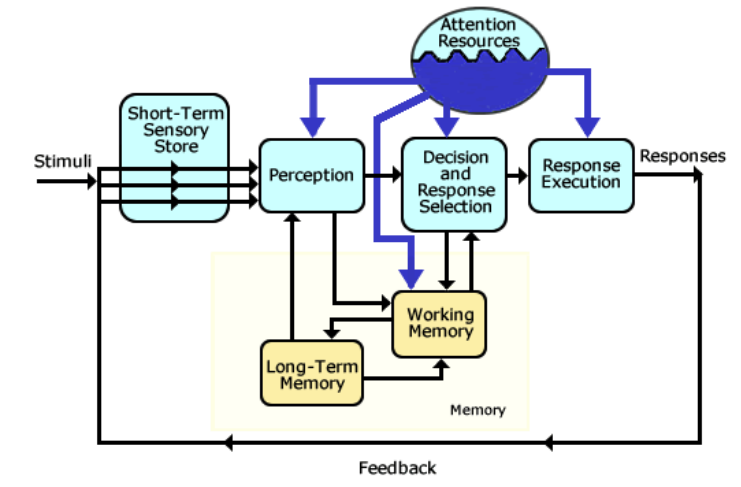
\includegraphics[width=.5\textwidth]{img/ch03_hip_overview}
	\caption{HIP -- Overview}
	\label{hip}
\end{figure} 

\subsection{Senses}
A sense is a system that consists of a sensory cell type (or group of cell types) that respond to a specific kind of physical energy, and that correspond to a defined region (or group of regions) within the brain where the signals are received and interpreted.\\
Six external senses: sight, hearing, touch, smell, taste, balance\\
Three internal senses: thermoception, nociception (for pain), proprioception 

\subsection{Short-Term Sensory Storage (STSS)}
Sensory Memory is the retention, for brief periods of time, of the effects of sensory stimulation.\\
$\rightarrow$ Collecting information for processing, holding it briefly while initial processing is going on, filling in the blanks when stimulation is intermittent.\\
STSS does not need explicit attention, it works pre-attentive and is not part of the conscious memory. Note that STSS != short term memory.\\
Two most important types of short-term sensory memory:
\begin{itemize}
\item echoic memory (lasts $\approx 2-10s$ after stimulus) $\rightarrow$ e.g. ``What did you say?''
\item iconic memory (lasts $\approx 0.5-1.0s$ after stimulus) $\rightarrow$ e.g. grid of letters
\end{itemize}

\subsection{Perception}
Human capability of information processing is limited! It is not only of interest, how much information is presented to a human, but
\begin{itemize}
\item how much information is transmitted from stimulus to response
\item capacity of the information channel
\item how rapidly information is transmitted (bandwidth)
\end{itemize}
Raw sensory data must be interpreted and given meaning. This process is called perception. It generally happens automatically (little attention needed) and fast (in contrast to cognitive processes).
\begin{itemize}
\item driven by sensory inputs $\rightarrow$ bottom-up
\item driven by long-term memory $\rightarrow$ top-down
\end{itemize}

\subsection{Attention}
Attention is the cognitive process of selectively concentrating on one aspect of the environment while ignoring other things. It is the crucial element for cognitive processes as
learning or task execution. Types of attention:
\begin{itemize}
\item selective attention: willingly select focus
\item focused attention: respond to external events
\item divided attention: simultaneous focusing on different events
\end{itemize}
\textbf{Allocation Model of Attention (Kahneman, 1973)}:
Limited amount of ``processing power'' at our disposal. Task execution depends on how much of our attention ``capacity'' we can spare on it.\\\\
\textbf{Controlled and Automatic Attention (Schneider and Shiffrin, 1977)}:
\begin{itemize}
\item Controlled processing makes heavy demands on attentional resources, is slow and limited in capacity, and involves consciously directing attention towards a task.
\item Automatic processing makes no demands on attentional resources, is fast, unaffected by capacity limitations, unavoidable and difficult to modify, and is not subject to conscious awareness
\end{itemize}
\textbf{Selective and Focused Attention}:
Concentration on one stimulus source needed for e.g. perception or learning (visual sampling or scanning). Being too selective is referred to as ``cognitive tunneling''.\\
Negative examples: selecting cues that stand out rather than useful ones (e.g. during a presentation/argumentation).\\
Humans have tendency to be distracted $\rightarrow$important e.g. for directing attention to warning/error messages\\
Differences in errors between selective attention and focused attention: intentional selection of the wrong source vs. unintentional external influences.\\\\
\textbf{Divided Attention}:
C.f. attention models. Limited attention capacity of humans, important e.g. for layout of instruments in a cockpit (see Gestalt laws). Differences in errors between focused attention and
divided attention: some of our attention is directed to stimuli we do not wish to process vs. our limit to attend to all stimuli we wish to process.\\
$\rightarrow$ Only a certain maximum of attention capacity can be divided to tasks!\\
Attention can be directed at a particular task and/or divided between a number of different tasks. Practice reduces the amount of attention required by a particular task (e.g. typing blindly on a keyboard while reading a text). Attention and awareness are closely linked.

\subsection{Vigilance}
Vigilance is an aspect of attention which refers to detecting a rare event or signal in a desert of inactivity or noise.
It means to detect signals over a long period of time which are intermittent, unpredictable, and infrequent, but it is known that they happen.\\
Examples of vigilance tasks: security inspector x-raying luggage, quality control in production\\
$\rightarrow$ vigilance level (steady-state level performance)\\
$\rightarrow$ vigilance decrement\\\\
\textbf{Paradigms}:
\begin{itemize}
\item free-response paradigm: a target event occurs at any time, non-events are not defined; example: power plant monitor supervision
\item inspection paradigm: events occur at fairly regular intervals; some are events, most are non-targets; example: quality control (most items are ok, only some have defects)
\item successive vigilance paradigm: target stimulus has to be remembered; successive events have to be compared to the target stimulus; example: detect if a color is darker than the initial target
\item simultaneous vigilance paradigm: all events/information needed for discrimination are present at the same time; example: compare many types of garment to a standard piece of fabric
\item sensory vigilance paradigm: signals represent changes in the auditory or visual intensity; example: color changes
\item cognitive vigilance paradigm: signals represent ``information'' (symbolic or alphanumeric stimuli); example: proofreading a manuscript
\end{itemize}

\subsection{Workload and Measurement -- Signal Decision Theory}
The SDT model assumes that there are two stages of information processing in the task of detection: Sensory evidence is aggregated concerning the presence or absence of the signal. A decision is made about whether this evidence indicates a signal or not.\\
Signal detection \& neural activity: External stimuli generate neural activity. On average, there will be more neural evidence when a signal is present than when it is absent.\\

Types of noise:
\begin{itemize}
\item internal (in our brain, e.g. firing rate of neurons varies for the same stimulus)
\item external (in the data) internal response (in the observer's brain)
\end{itemize}
The probability distributions for internal response can be different for noise and for signal! Internal response as neural activity resulting from a stimulus:
\begin{figure}[h!]
	\centering
	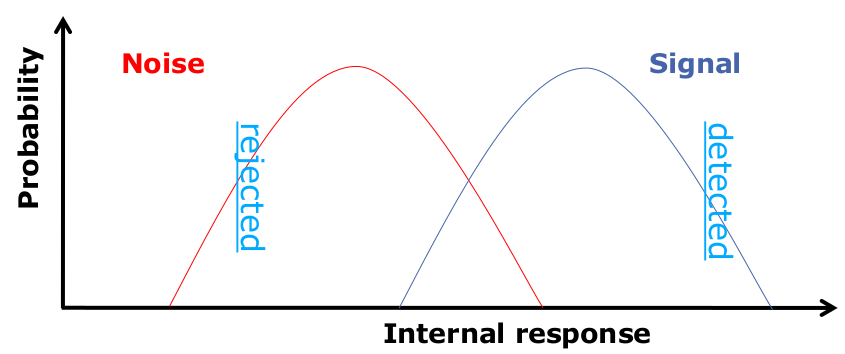
\includegraphics[width=.5\textwidth]{img/ch03_std.png}
	\caption{}
	\label{std}
\end{figure} 
\begin{figure}[h!]
	\centering
	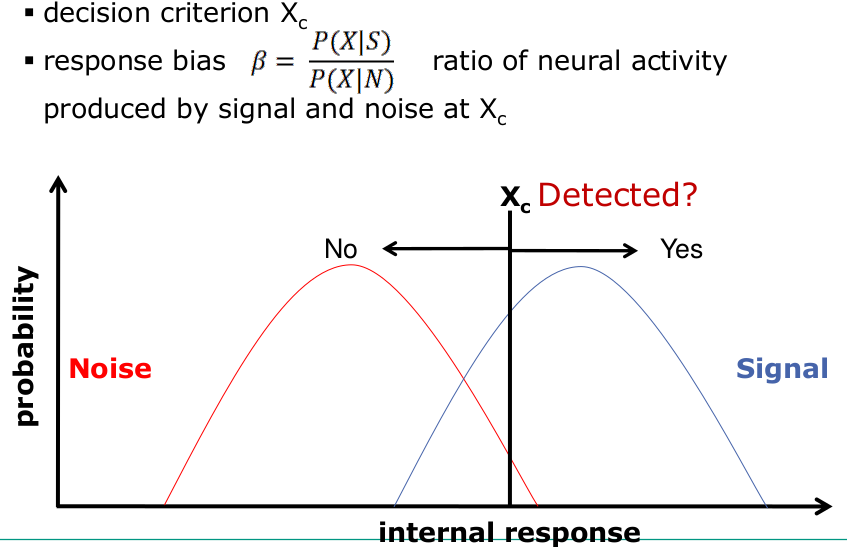
\includegraphics[width=.5\textwidth]{img/ch03_std1.png}
	\caption{}
	\label{std1}
\end{figure} 
\begin{figure}[h!]
	\centering
	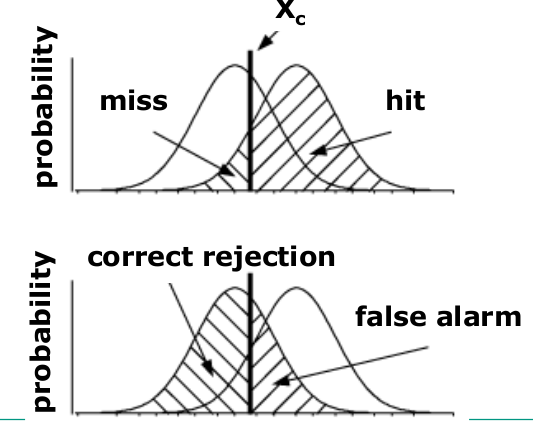
\includegraphics[width=.3\textwidth]{img/ch03_std2.png}
	\caption{signal classifications revisited: hit, miss, false alarm and correct rejection}
	\label{std2}
\end{figure} 
Optimal beta (bias) should be set where the probability of signal and noise are equal. $\beta_{opt}$ tells us where the bias should be, while $\beta$ tells
us where the bias really is. $\beta_{opt} = \frac{P(N)}{P(S)}$\\
Usually, humans adapt ``their'' beta not enough (too conservative or too risky):
\begin{itemize}
\item[$\rightarrow$] Over-estimation of rare events
\item[$\rightarrow$] Under-estimation of frequent events
\item[$\rightarrow$] ``Sluggish beta'' refers to highly focused attention processes, rare attention or sub-conscious processes underestimate rare events.
\end{itemize}
\textbf{Sensitivity} (d’) is the resolution of the detection mechanism. It refers to the separation of noise and signal distributions along the $X$-axis and corresponds to the separation of the means of the two distributions.
\begin{figure}[h!]
	\centering
	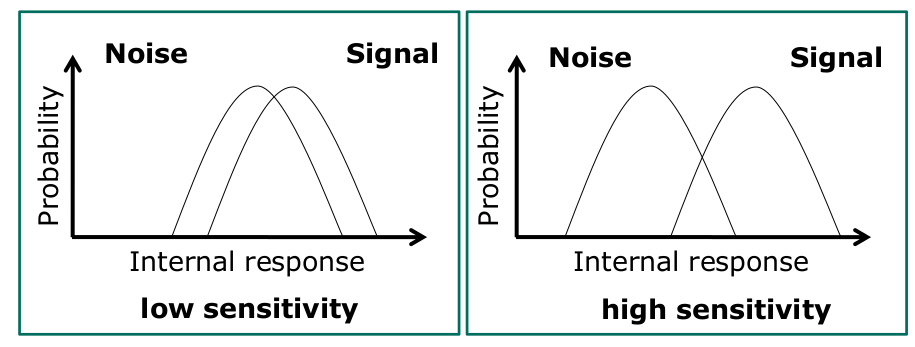
\includegraphics[width=.5\textwidth]{img/ch03_std3.png}
	\caption{Sensitivity}
	\label{std3}
\end{figure} 

\subsection{Memory}
Human memory consists of two major components: Working memory (formerly: short-term memory) and long-term memory. Memory ``processes'' include recall, recognition, chunking and rehearsal. Human memory is multi-modal! The brain makes up 2\% of a person's weight. It consumes 20\% of the body's energy, even at rest. Brain energy consumption is 10 times the rate of the rest of the body per gram of tissue. Average power consumption of a typical adult lays at 
100 Watts brain consumes 20\% (20W) of this.\\ \\
\textbf{Working Memory}:
\begin{itemize}
\item Memory storage for up to 30 seconds, after that short period, the contents decay or are displaced.
\item rapid access: $\approx$ 70ms access time
\item storage size: 3-4 ``chunks'' (NOT: 7+--2 elements!)
\item it is easy to overwrite the contents (intentionally and
unintentionally!)
\item can store two different types of data at the same time: visual information (visuo-spatial sketchpad) \& verbal information (articulatory loop)
\item to maintain the contents of working memory: rehearsal is needed
\item to persistently store information from working memory: move it to long-term memory
\end{itemize}
Types of WM:
\begin{itemize}
\item Verbal: Phonological Store\\
$\rightarrow$ Retrieval: Articulatory loop\\
$\rightarrow$ ``Programmed'' and associated by words written, spoken (the latter are simpler to remember)
\item Visual; Visuospatial Sketchpad, stored often in form of images
\item Operate in parallel, but there is only a restricted number of attention levels
\end{itemize}
\textbf{Long-Term Memory}:
\begin{itemize}
\item ``unlimited'' in capacity
\item lasts from a few minutes to life time
\item slow access: 100ms seconds access time
\item multi-modal memory: smell as strong trigger to long-term memory (sound as most efficient cue for working memory)
\item three types (could be clustered otherwise, depending on psychological model): episodic – serial memory of events, procedural – knowledge of how to do things, semantic – structured memory of facts, concepts, skills
\item semantic LTM ($\rightarrow$ relationships between bits of information, inference through inheritance) derived from episodic LTM
\item Forgetting: decay (information is lost gradually, but very slowly), interference (retroactive interference: new information replaces old, proactive inhibition: old may interfere with new);  affected by emotion (can subconsciously `choose' to forget)
\end{itemize}
\begin{figure}[h!]
	\centering
	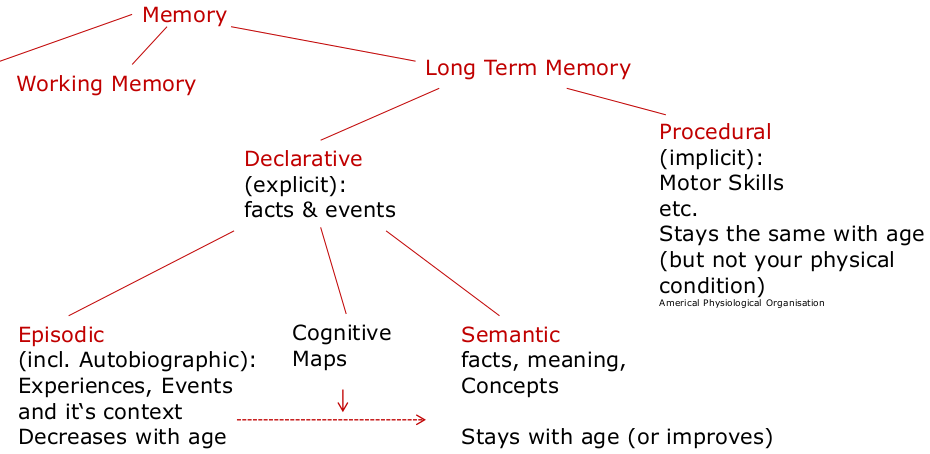
\includegraphics[width=.5\textwidth]{img/ch03_mem.png}
	\caption{}
	\label{Memory Model}
\end{figure} 
Long Term Memory Processes:
\begin{itemize}
\item Encoding is the process by which information is stored in memory.
\item Retrieval is the means by which memories are recovered from long-term storage.
\item Forgetting is the name of a number of different possible processes by which we fail to recover information.
\item recall (``Erinnerung''): active memory search to retrieve a particular piece of information
\item recognition (``Wiedererkennung''): searching the memory and deciding whether the retrieved piece of information matches a given information; recognition is generally easier and quicker than recall!
\item[$\rightarrow$] Icons often use metaphor to recall an associated object or activity\footnote{Horton‘s checklists for icons: Understandable, Familiar, Unambiguous, Memorable, Informative (concept important?), few (<20), distinct, attractive, legible (tested in all view contexts), compact (means minimal), coherent (can be separated from other icons and the background), extensible (means size scalable)}
\item rehearsal: There is no direct link from perception to LTM! The process of repeating information in working memory. This facilitates the short-term recall of information and its transfer to long-term memory. The amount stored is proportional to the number of rehearsals!
\item chunking: grouping of items into more meaningful units
\end{itemize}

\subsection{Memory Design Guidelines}\footnote{Guideline: specific and practical rules for solving problems of UI design;\\ Principles: help for analyzing and comparing design alternatives;\\
Theories and Models: describe objects and actions with consistent terminology and give a comprehensible explanation of connections}
\begin{itemize}
\item[M1:] Organize information into a small number of ``chunks''.
\item[M2:] Try to create short linear sequences of tasks.
\item[M3:] Use persistence, so do not flash important information onto the screen for brief time periods.
\item[M4:] Do not ``overwrite'' the contents of working memory by giving additional tasks to the user.
\item[M5:] Organize data fields to match user expectations or to organize user input (e.g. the automatic formatting of phone numbers)
\item[M6:] Provide reminders or warnings of the state the user has reached in an operation.
\item[M7:] Provide ongoing feedback on what is happening and/or what has just happened.
\item[M8:] The user interface should behave in consistent ways at all the times for all screens.
\item[M9:] Terminology, icons and the use of color should be consistent between screens.
\end{itemize}

\subsection{Decision Making}
Semantic coding: without memory, there is no ``thinking'' or decision-making! After the perception of the stimulus, a response needs to be selected.\\
Automatic vs. controlled decisions:
\begin{itemize}
\item automatic($\rightarrow$ fast): little or no attention required, learned reflexes or behavior, a long-term memory procedure is executed nearly automatically in response to the stimulus
\item controlled ($\rightarrow$ slow): attention required, typically conscious of thoughts, interaction with WM and LTM systems
\end{itemize}
\subsection{Response and Feedback}
After a decision has been made, it has to be executed by complex motor movements.\\
Feedback-loop: we observe the consequences of our actions, producing closed-loop feedback $\rightarrow$ the model is circular rather than linear (\autoref{hip})!

\subsection{HIP by Numbers}
\textbf{CMN-Model} (Card, Moran \& Newell, 1983):\\
Three interacting subsystems, each with processor \& memory and described by parameters; serial \& parallel processing
\begin{enumerate}
\item Perceptual processor: receives sensory input (audio \& visual), codes info symbolically, output into audio \& visual image storage (WM buffers)
\item Cognitive processor: input from sensory buffers, can access LTM to determine response according to previously stored info, output response into WM
\item Motor processor: input response from WM, carry out response
\end{enumerate}
Subsystem interactions in terms of input/output. Processing:
\begin{itemize}
\item serial action: e.g. pressing key in response to light
\item parallel perception: e.g. driving, reading signs \& hearing
\end{itemize}
\textbf{Parameters} (based on empirical data):\\
Processors have: cycle time ($\tau$)\\
Memories have: storage capacity ($\mu$), decay time of an item ($\delta$), info code type ($\kappa$, physical, acoustic, visual \& semantic)
\begin{itemize}
\item Processor cycle time: $\tau_{per} = 100ms$, $\tau_{cog} = 70ms$, $\tau_{mot} = 70ms$ $\rightarrow$ total time: $\tau_{per} + \tau_{cog} + \tau_{mot}$
\item Visual image store:  $\mu_{per} =$17 letters (visual) / 5 letters (auditive), $\mu_{WM} =$3-7 chunks
\item Decay time (half-life index): $\delta_{per}=200ms$ (visual), $\delta_{per}=1500ms$ (auditive); $\delta_{WM}=7s$ (for 3 chunks), $\delta_{WM}=73s$ (for 1 chunk) 
\item Info code type: $\kappa$ = physical $\rightarrow$ physical properties of visual stimulus (e.g. intensity, color, curvature, length)
\end{itemize}
Principle of Operation -- Power Law of Practice: task time on the $n^th$ trial $T_n = T_1n^{-0.4}$
$\rightarrow$ you get faster the more times you do it, applies to skilled behavior (perceptual \& motor) but not to knowledge acquisition\\
$\Rightarrow$ These numbers are used later for the interaction design models